%%%%%%%%%%%%%%%%%%%%%%%%%%%%%%%%%%%%%%%%%%%%%%%%%%%%%%%%%%%%%%%%%%%%%%
% Problem statement
\begin{statement}[
  problempoints=100,
  timelimit=1 sekunda,
  memorylimit=512 MiB,
]{3D Histogram}

\textbf{Gospodin Malnar (preko telefona):} Čuj, morao sam pod okriljem noći
lijepiti neke plakate tu po Zagrebu. Naišao sam tako na jednu ogradu koja se
sastojala od dasaka različitih visina pa sam razmišljao kako izračunati koji
je najveći mogući plakat koji tamo mogu zalijepiti. Što misliš, je li to
dobar zadatak za HIO?

\textbf{Stručni suradnik:} Što? Lijepio si plakate usred noći?! Uglavnom,
zadatak ti nije ni za logo ligu, na kampovima već i osnovnoškolcima objašnjavamo
kako pronaći najveći pravokutnik u histogramu. Standardna fora s monotonim
stackom.

\textbf{Gospodin Malnar:} Ma dobro, promijeni ga malo, neka ispišu rješenje za
svaki prefiks ili tako nešto, bit će im dovoljno teško.

\textbf{Stručni suradnik:} To je bilo ove godine na studentskom, nezgodan
zadatak, svede se na \textit{Harbingers} trik, ali sad su ga svi već
vidjeli.

\textbf{Gospodin Manlar:} Siguran si da ga ne možemo nikako iskoristiti.

\textbf{Stručni suradnik:} Ma da, iscrpili smo zadatke s histogramima. HONI
  2010/2011 (Tabovi), HONI 2015/2016 (Poplava), HONI 2017/2018 (Krov), izborne
  pripreme 2018.\ (Histogram)... Trebam li još nabrajati?

\textbf{Gospodin Manlar:} A što ako je histogram trodimenzionalan?

\textbf{Stručni suradnik:} Hmm...

Zadan je 3D histogram koji se sastoji od $N$ kvadara širokih $1$ metar koji se
nalaze jedan do drugog. Visina $i$-tog kvadra iznosi $a_i$ metara, a njegova
dužina iznosi $b_i$ metara. Odnosno, nacrt (pogled sprijeda) 3D histograma
jest histogram sa stupcima visina $a_1$, $a_2$, \dots, $a_N$, dok je njegov
tlocrt (pogled odozgo) histogram sa stupcima visina $b_1$, $b_2$, \dots,
$b_N$.


Odredite kvadar maksimalnog obujma kojeg je moguće u potpunosti smjestiti unutar
zadanog 3D hisograma. Stranice tog kvadra moraju biti paralelne sa stranicama
kvadara koji čine 3D histogram.

%%%%%%%%%%%%%%%%%%%%%%%%%%%%%%%%%%%%%%%%%%%%%%%%%%%%%%%%%%%%%%%%%%%%%%
% Input
\subsection*{Ulazni podaci}
U prvom je retku prirodan broj $N$ iz teksta zadatka.

U $i$-tom od sljedećih $N$ redaka nalaze se brojevi $a_i$ i $b_i$ iz
teksta zadatka.

%%%%%%%%%%%%%%%%%%%%%%%%%%%%%%%%%%%%%%%%%%%%%%%%%%%%%%%%%%%%%%%%%%%%%%
% Output
\subsection*{Izlazni podaci}
Ispišite obujam traženog kvadra u kubnim metrima.

%%%%%%%%%%%%%%%%%%%%%%%%%%%%%%%%%%%%%%%%%%%%%%%%%%%%%%%%%%%%%%%%%%%%%%
% Scoring
\subsection*{Bodovanje}
{\renewcommand{\arraystretch}{1.4}
  \setlength{\tabcolsep}{6pt}
  \begin{tabular}{ccl}
 Podzadatak & Broj bodova & Ograničenja \\ \midrule
  ?? & ?? &  \\
\end{tabular}}

%%%%%%%%%%%%%%%%%%%%%%%%%%%%%%%%%%%%%%%%%%%%%%%%%%%%%%%%%%%%%%%%%%%%%%
% Examples
\subsection*{Probni primjeri}
\begin{tabularx}{\textwidth}{X'X'X}
\sampleinputs{test/3dhistogram.dummy.in.1}{test/3dhistogram.dummy.out.1} &
\sampleinputs{test/3dhistogram.dummy.in.2}{test/3dhistogram.dummy.out.2} &
\sampleinputs{test/3dhistogram.dummy.in.3}{test/3dhistogram.dummy.out.3}
\end{tabularx}

\textbf{Pojašnjenje prvog probnog primjera:} donja slika odgovara prvom
probnom primjeru. Najveći se kvadar dobiva koristeći dio prvog i dio drugog
kvadra iz ulaza, a širok je $2$ metra, visok je $4$ metra i dug $3$ metra. Dakle
ima obujam od $2 \cdot 4 \cdot 3 = 24$ kubna metra.

\begin{figure}[H]
\centering
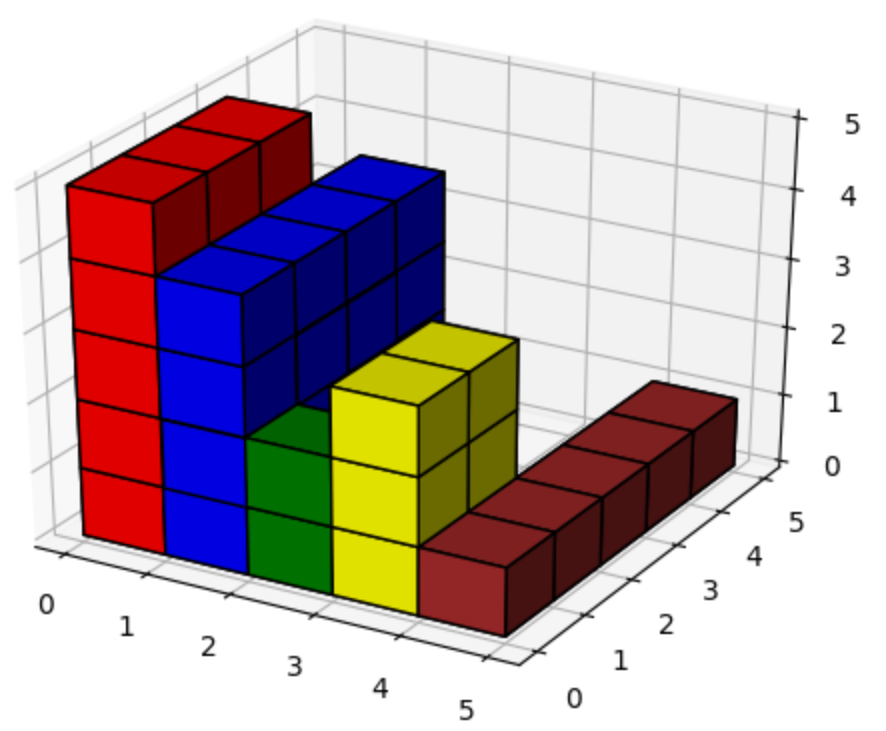
\includegraphics[width=0.5\textwidth]{img/3dhistogram_skica.png}
\end{figure}

%%%%%%%%%%%%%%%%%%%%%%%%%%%%%%%%%%%%%%%%%%%%%%%%%%%%%%%%%%%%%%%%%%%%%%
% We're done
\end{statement}

%%% Local Variables:
%%% mode: latex
%%% mode: flyspell
%%% ispell-local-dictionary: "croatian"
%%% TeX-master: "../hio.tex"
%%% End:
